%! TeX program = lualatex
\documentclass[11pt,ngerman]{scrartcl}

% standard packages
\usepackage[utf8]{inputenc}  % input in UTF-8
\usepackage[T1]{fontenc}  % output in T1 fonts (westeuropäische Codierung)
\usepackage{lmodern}  % latin modern fonts
\usepackage[ngerman]{babel}  % deutsches Sprachpaket, neue Rechtschreibung

% Seitensetup
\usepackage{scrlayer-scrpage}  % Seitenformatierung durch KOMA-interne Optionen
\usepackage[top=4cm, bottom=4cm]{geometry}  % Seitengeometrie (kann durch KOMA ersetzt werden, hab ich aber nicht geschafft)
\usepackage[hypcap=false]{caption, subcaption}  % caption editing - hypcap warning with hyperref
\usepackage{array}  % table editing

% additional packages
\usepackage{amsmath, amssymb, amstext}  % math packages (American Math Society)
\usepackage{bm}
\usepackage{icomma}  % Kommata in Dezimalzahlen verursachen keinen Abstand mehr
\usepackage{graphicx}  % Bilder einfügen
\usepackage{float} %Bilder placement
\usepackage{pdfpages}  % PDF als vollständige Seiten einfügen
\usepackage{lastpage}  % referenziert die letzte Seite
\usepackage[separate-uncertainty=true]{siunitx}  % bessere Darstellung von Einheiten
\usepackage{makecell} %Dicke Tabellenstriche
\usepackage{longtable}
\usepackage{booktabs}
%\usepackage{datatool}
\usepackage[hidelinks]{hyperref}  % hyperref verlinkt Referenzen - hidelinks entfernt borders um links

% package setups
% Kopf- und Fußzeile durch KOMA
\pagestyle{scrheadings}  % KOMA darf entscheiden
\clearpairofpagestyles  % reset
\setkomafont{pageheadfoot}{\normalfont}  % Standardschrift in Kopf- und Fußzeile
\captionsetup{format=plain, font=small, labelfont=bf} %Better caption, Abbildung ist FETT
%\setlength{\headheight}{27.2pt}  % benötigte Höhe Kopfzeile (warning von scrlayer-scrpage, wird aber automatisch so gerendert, falls diese Option weggelassen wird)
\ihead{Abbe-Theorie}  % Kopf links %Todo Titel ändern
\chead{\textsc{Philipp} Maximilian \\ \textsc{Stark} Matthias}  % Kopf Mitte %Todo Name ändern
\ohead{08 Oktober 2021}  % Kopf rechts %Todo Datum ändern
\cfoot{\pagemark \, / \pageref{LastPage}}  % Fuß Mitte

% Table of Contents
\DeclareTOCStyleEntry{dottedtocline}{section}  % KOMA intern - Inhaltsverzeichnis mit Punkten (nur sections)

%Overbar setup
\newcommand{\overbar}[1]{\mkern 1.5mu\overline{\mkern-1.5mu#1\mkern-1.5mu}\mkern 1.5mu}
% SI
\sisetup{locale = DE}  % deutschsprachige SI-Konvention
\sisetup{per-mode = fraction}
\DeclareSIUnit\px{px}
\DeclareSIUnit\strich{|||}

% citation
\usepackage{csquotes}
\usepackage[backend=biber]{biblatex}
\addbibresource{quincke-kundt.bib} %Todo .bib befüllen zb.: mit JabRef (Empfehlung der Redaktion)

%Eigene Commands
\newcommand{\der}[2]{\frac{\mathrm{d}#1}{\mathrm{d}#2}}
\newcommand{\pder}[2]{\frac{\partial #1}{\partial #2}}

\begin{document}
\includepdf{Deckblatt_Stark.pdf}
\tableofcontents
\newpage

\section{Aufgabenstellung\label{Auf0}}

Zunächst soll der Zusammenhang zwischen der Auflösung des Bildes eines
Spaltgitters und der Anzahl der transmittierten Beugungsordnungen untersucht
werden.

\noindent Weiters soll auch das Auflösungsvermögen einer Linse in Abhängigkeit
ihrer numerischen Apertur (N.A.) für zwei unterschiedliche Wellenlängen
bestimmt werden. \cite{abbevorlage}



\section{Voraussetzungen und Grundlagen}  % (fold)
\label{sec:voraussetzungen_grundlagen}

Wenn Überlagerungsprozesse von Wellen abgebildet werden, ist es oftmals
relevant, was die Grenzen des Auflösungsvermögens dieser Prozesse sind.
Diese Überlegungen finden Anwendungen bei Mikroskopie, Ultrasonographie
und vielen weiteren Gebieten \cite{wiki_aufl_2020}.
Dieses Experiment beschäftigt
sich mit dem Auflösungsvermögen verschiedener Wellenlängen bei der
Lichtmikrokopie.

\noindent Die Abbe'sche Abbildungstheorie liefert eine Erklärung für diese Frage. Abbe
stellte fest, dass das Auflösungsvermögen $d$ nur von dem Öffnungswinkel
abhängig ist. Weiters sei das Auflösungsvermögen invers-proportional zum Sinus vom
Halben Öffnungswinkel $\alpha$ also:

\begin{equation}
	d \propto \frac{1}{\sin(\alpha)}
	\label{eq:abbepropo}
\end{equation}

\vspace{2mm}

\noindent Zudem postulierte Abbe, dass, wenn das erste Nebenmaximum nicht mehr vom
Objektiv aufgefangen werden kann, das Objekt nicht mehr aufgelöst werden kann.\cite{demtroder2018ex2}

\noindent Die Abbe-Theorie beruht auf dem Prinzip, dass jedes Objekt Beugungseffekt hervorruft und
die Information des Bildes auf die Beugungsmaxima aufgeteilt wird, dies wird für eine Gitterlinie
in \autoref{fig:beugungseffekt} veranschaulicht.\cite{demtroder2018ex2}

\begin{figure}[H]
	\begin{center}
		\includegraphics[width=0.5\textwidth]{./pics/beugungsphaenomen.pdf}
	\end{center}
	\caption{Veranschaulichung von Beugungseffekten bei einem einzelnen Gitterstrich \cite{SchweizerAbbe}}
	\label{fig:beugungseffekt}
\end{figure}

\noindent Sind nun mehrere Objekte, die Beugungseffekte hervorrufen, vorhanden, überlagern sich dessen
Wellen und erzeugen je nach Abstand der Objekte unterschiedliche überlagerte Wellenfunktionen.

\vspace{2mm}

\noindent Im Folgenden sind verschiedene überlagerte Wellen, bei verschiedenen Abständen der
Objekte, dargestellt.

\vspace{2mm}

\begin{minipage}{\textwidth}
	\begin{minipage}[t]{0.5\textwidth}
		\centering
		\includegraphics[width=\textwidth]{pics/0ordnung}
		\captionbelowof{figure}{Abbildung der Linse bei der \newline nur die nullte
			Beugungsordnung vom \newline Objektiv erfasst wird \cite{SchweizerAbbe}}
		\label{fig:0ordnung}
	\end{minipage}
	\vspace{2mm}
	\begin{minipage}[t]{0.50\textwidth}
		\centering
		\includegraphics[width=\textwidth]{pics/1ordnung}
		\captionof{figure}{Abbildung der Linse bei der \newline die nullte und
			erste Beugungsordnung vom \newline Objektiv erfasst werden
			\cite{SchweizerAbbe}}
		\label{fig:1ordnung}
	\end{minipage}
	\vspace{1em}
\end{minipage}

\begin{minipage}{\textwidth}
	\begin{minipage}[t]{0.5\textwidth}
		\centering
		\includegraphics[width=\textwidth]{pics/1ordnung_grenzfall}
		\captionbelowof{figure}{Abbildung der Linse beim \newline Grenzfall, sodass
			die erste Beugungsordnung \newline gerade nicht vom Objektiv erfasst wird
			\cite{SchweizerAbbe}}
		\label{fig:1ordnung_grenzfall}
	\end{minipage}
	\vspace{2mm}
	\begin{minipage}[t]{0.50\textwidth}
		\centering
		\includegraphics[width=\textwidth]{pics/3ordnung}
		\captionof{figure}{Abbildung der Linse bei der \newline die
			Beugungsordnungen bis zur dritten Ordnung \newline vom Objektiv erfasst
			werden \cite{SchweizerAbbe}}
		\label{fig:}
	\end{minipage}
	\vspace{1em}
\end{minipage}


\noindent Bei einem Mikroskop ruft das Objekt, welches untersucht wird, Beugungseffekte,
genau wie der Strich zuvor, hervor. Der Einfachheit halber wird die Funktionsweise
eines Mikroskops anhand eines Gitters erklärt. Die \autoref{fig:1ordnung_grenzfall} stellt
den Grenzfall der Auflösung dar, anhand dem das Auflösungsvermögen $d$
errechnet werden kann.

\begin{align}
	d \sin(\alpha) & = k \frac{\lambda}{n} \quad k \in \mathbb{N}                     \\
	d              & = \frac{\lambda}{n \sin(\alpha)}    \label{eq:abbe_ohne_beugung} \\
\end{align}


\noindent Weil bei der Mikroskopie auf Grund von Beugung das Rayleigh Kriterium
\cite{wiki_rayleigh_2021} verwendet wird, gelangt man durch einsetzen von der
Definition von dem Durchmesser der Numerischen Apertur $d = 2\, \mathrm{N.A.}$
auf folgende \autoref{eq:aufl_theo}:

\begin{equation}
	d \approx \theta = 1.22 \frac{\lambda}{2 \mathrm{N.A.}}
	\label{eq:aufl_theo}
\end{equation}


\begin{center}
	\begin{minipage}[t]{0.5\textwidth}
		\centering
		\includegraphics[width=\textwidth]{pics/abbe_ordnungen}
		\captionbelowof{figure}{Skizze für die Anzahl der Ordnungen, die noch erfasst und auf den Brennpunkt abgebildet werden}
		\label{fig:abbildung_brennebene}
	\end{minipage}
\end{center}


\noindent Wie in \autoref{fig:abbildungs_skizze} und \autoref{fig:na_naherung} ersichtlich lässt sich die Numerische Apertur mittels der Winkelfunktionsnäherungen
wie folgt bestimmen:

\begin{equation}
	\mathrm{N.A.} = \frac{r}{f}
	\label{eq:na_approx}
\end{equation}

\begin{center}
	\begin{minipage}[t]{0.50\textwidth}
		\centering
		\includegraphics[width=\textwidth]{pics/abbeabbildung_skizze}
		\captionof{figure}{Abbildungsskizze}
		\label{fig:abbildungs_skizze}
	\end{minipage}
\end{center}

\begin{center}
	\begin{minipage}[t]{\textwidth}
		\includegraphics[width=\textwidth]{b}
		\captionof{figure}{Skizze für die Näherung für die Berechnung der N.A. \cite{abbevorlage}\cite{demtroder2018ex2}}
		\label{fig:na_naherung}
	\end{minipage}
\end{center}

\noindent Um von der in der Tabelle gegebenen räumlichen Frequenz $\xi$ auf den Abstand zwischen zwei Gitterstrichen
zu kommen verwendet man folgende \autoref{eq:aufl_durch_xi}:
\begin{equation}
	d = \frac{1}{\xi}
	\label{eq:aufl_durch_xi}
\end{equation}

\noindent Folgende \autoref{eq:intensity_distribution} für Intensitätsverteilung in Abhängigkeit von
$\lambda$ der Wellenlänge, $b$ der Spaltbreite, $g$ dem Spaltabstand, $N$ der Anzahl an Spalten und
dem Beugungswinkel $\phi$ wurde aus dem Demtröder entnommen \cite{demtroder2018ex2}:

\begin{equation}
	I(\phi) = I_0 \left(\frac{\sin(\pi \frac{b}{\lambda} \sin(\phi))}{\pi \frac{b}{\lambda}\sin(\phi)} \frac{\sin(N \pi \frac{g}{\lambda} \sin(\phi))}{\sin(\pi \frac{g}{\lambda} \sin(\phi))}\right)^2
	\label{eq:intensity_distribution}
\end{equation}

\noindent Wird die Spaltbreite $b$ gleich dem halben Spaltabstand $g$ gesetzt $b = \frac{g}{2}$ und \autoref{eq:intensity_distribution} über
den Beugungswinkel $\phi$ aufgetragen und auf $I_0$ normiert erhält man folgende \autoref{fig:intensitat}:

\begin{center}
	\begin{minipage}[t]{\textwidth}
		\includegraphics[width=\textwidth]{interferenz}
		\captionof{figure}{Intensitätsverlauf des Beugungsbilds mit Spaltbreite
			entspricht dem halben Spaltabstand \cite{demtroder2018ex2}}
		\label{fig:intensitat}
	\end{minipage}
\end{center}

\noindent Dabei wird ersichtlich, dass die Beugungsmaxima der geraden Ordnungen auf Grund von destruktiver Interferenz verschwinden.

\vspace{2mm}

\noindent Um zu sehen wie sich die Unsicherheit der Messungen bis in die Ergebnisse
fortplanzt, ist \autoref{eq:Unsicherheitsfortpflanzung} verwendet worden.
Die Grundlagen dieser Gleichung stammen von den Powerpointfolien von
GUM.\cite{WolfgangKessel2004} Die Verallgemeinerung ist von Wikipedia entnommen
worden \cite{2020Fehler}.
Für die Auswertung ist die Progammiersprache Python im speziellen das
Packet \verb#scipy#, zur Hilfe genommen worden.

\begin{equation}
	\label{eq:Unsicherheitsfortpflanzung}
	V_y = J(x) \cdot V_x \cdot J^{T}(x)
\end{equation}

\noindent Wobei $V_y$ und $V_x$ die Kovarianzmatrizen von den Vektoren $\bm{y}$ und $\bm{x}$ sind.
$\bm{x}$ ist der Vektor der Eingangsvariablen und $\bm{y}$ ist der Vektor der Ausgangsvariablen.
$J$ ist die Jakobimatrix der vektorwertigen Funktion $\bm{y} = \vec{F}(\bm{x})$.
So lassen sich die Komponenten der Matrix relativ einfach anschreiben $J_{ij}(x) = \frac{\partial{y_i}}{\partial{x_j}}(x)$.
Damit man die Unsicherheit der einzelnen Variablen $y_i$ bekommt, muss nur die Quadratwurzel des i-ten Diagonalelementes der
$\bm{y}$-Kovarianzmatrix genommen werden $u_i= \sqrt{\mathrm{diag}(V_y)_i}$.
Da in diesem Experiment meistens nur skalare Funktionen untersucht werden, vereinfacht
sich die \autoref{eq:Unsicherheitsfortpflanzung} dramatisch und die Unsicherheit
der Variable $y$ lässt sich einfach so berechnen:

\begin{equation}
	\label{eq:graduncentainty}
	u_y = \sqrt{\mathrm{grad} y^T \cdot V_x \cdot \mathrm{grad} y}
\end{equation}

\vspace{5mm}

\newpage
\section{Versuchsanordnung}\label{sec:Versuchsanordnung}

Der schematisch Aufbau des Versuchs ist in folgender Skizze ersichtlich:

\begin{center}
	\begin{minipage}[t]{\textwidth}
		\includegraphics[width=\textwidth]{skizze}
		\captionof{figure}{Skizze der Versuchsanordnung }%beschr. der V:
		\label{fig:skizze}
	\end{minipage}
\end{center}

\noindent Der Laserstrahl trifft, durch die Linse L1 gebündelt, auf das Testobjekt T, welches später noch genauer beschrieben wird. Am Filterrad F kann ausgewählt werden, ob der Laser durch die Apparatur scheint, oder einer der beiden LEDs verwendet wird. Bei der Abbildungslinse L2 handelt es sich um ein achromatisches Linsenpaar, um den Abbildungsfehler zu minimieren. Am Filterrad B kann mithilfe verschiedener Lochblenden die nummerische Apertur (N.A.) variiert werden. Die letzte Linse L3 ist klappbar angeordnet, wodurch an der Kamera wahlweise entweder das Beugungsbild oder das Bild des Objekts aufgenommen werden kann.

\noindent Die Linse L3 ist dabei genau so angeordnet, dass der Auflösungsfehler der Kamera vernachlässigbar klein ist.

\newpage

\noindent Die genaue Versuchsanordnung ist in \autoref{fig:aufbau} ersichtlich.

\begin{center}
	\begin{minipage}[t]{0.7\textwidth}
		\includegraphics[width=\textwidth]{abbe}
		\captionof{figure}{Versuchsanordnung}
		\label{fig:aufbau}
	\end{minipage}
\end{center}

\noindent Das verwendete Testobjekt ist in \autoref{fig:objekt} ersichtlich.

\begin{center}
	\begin{minipage}[t]{0.7\textwidth}
		\includegraphics[width=\textwidth]{objekt}
		\captionof{figure}{verwendetes Testobjekt \cite{abbevorlage}}
		\label{fig:objekt}
	\end{minipage}
\end{center}

\noindent Es handelt sich dabei um eine Anordnung aus horizontalen und
vertikalen Balken, bei denen jeweils ihr Abstand und die Breite der Striche
gleich groß sind. Mit der genauen Zuordnung der entsprechenden Gruppen und
Element Nummer kann anhand folgender Tabelle in \autoref{fig:tab} die Auflösung
eines optischen Geräts bestimmt werden. Dabei wird für die Räumliche Frequenz
der entsprechende Wert aus der Tabelle verwendet, der der entsprechenden
Gruppen und Elementnummer entspricht.

\begin{center}
	\begin{minipage}[t]{\textwidth}
		\includegraphics[width=\textwidth]{tabelle}
		\captionof{figure}{Tabelle mit den Räumlichen Frequenzen für die entsprechende Gruppen und Elementnummer \cite{abbevorlage}}
		\label{fig:tab}
	\end{minipage}
\end{center}

\vspace{5mm}

\section{Geräteliste}

Für die Messungen wurden folgende Geräte verwendet:
%Beispiel Tabelle 
\captionof{table}{Verwendete Geräte \newline $\Delta \dots$ Unsicherheit der Geräte}
\begin{center}
	\begin{tabular}{|c|c|c|c|} \hline
		\textbf{Gerät}      & \textbf{Typ}     & \textbf{Hersteller}      & $\Delta$ \\ \hline
		Linse 1             & f = 200 mm       &                          &          \\ \hline
		Linse 2             & f = 60 mm        &                          &          \\ \hline
		Linse 3             & f = 50 mm        &                          &          \\ \hline
		Helium-Neon Laser   & 632.8 nm         & Edmund Industrial Optics &          \\ \hline
		blaue LED           & 470 nm           &                          & 5 nm     \\ \hline
		rote LED            & 635 nm           &                          & 5 nm     \\ \hline
		Kamera              & DMK 42AUC03      & Imagingsource            &          \\ \hline
		Testobjekt          & 1951 USAF Target &                          &          \\ \hline
		Auswertungsprogramm & IC Capture       & The Imaging Source, LLC  &          \\ \hline
		Blende              &                  &                          &          \\ \hline
		Gestell             &                  &                          &          \\ \hline
	\end{tabular}
\end{center}

\newpage

\section{Versuchsdurchführung \& Messergebnisse}\label{sec:Versuchsdurchführung}

%\subsection{Programmeinstellungen}


\subsection{Zusammenhang zwischen der Auflösung und der Anzahl der Bergungsordnungen}

\noindent Zunächst werden die Linse L3 aus der Apparatur entfernt und am Testobjekt T die vertikalen Balken der dritten Gruppe und des vierten Elements, mithilfe von 2 Mikrometerschrauben, zentriert ausgerichtet. Durch vorsichtiges Verschieben, mithilfe eines Schraubmechanismus, wird nun das Bild, der zuvor erwähnten 3 Balken, am Computer scharfgestellt. Hierfür wird das Licht der roten oder blauen LED Lampen verwendet. Ist dies geschehen, wird das Filterrad F wider auf die Position gebracht, um das Laserlicht durch den Aufbau zu lassen.

\vspace{2mm}

\noindent Nun wird mithilfe der Computersoftware ``IC Capture`` die ``Exposure`` geändert, was der Belichtungszeit entspricht. Dabei ist zu beachten, dass am rechten Rand der angezeigten Grafik, die in \autoref{fig:graf} sichtbar ist, ein gelber Balken angezeigt wird. Dies bestätigt, dass die Belichtungsparameter richtig eingestellt sind.

\begin{center}
	\begin{minipage}[t]{0.7\textwidth}
		\includegraphics[width=\textwidth]{graf}
		\captionof{figure}{Grafik mit gelben Balken am Rand}
		\label{fig:graf}
	\end{minipage}
\end{center}

\noindent Wenn die Helligkeit richtig eingestellt ist, ist nun in der Software folgendes Bild aus \autoref{fig:bild} sichtbar. Wird nun die Linse L3 wieder in die Apparatur gegeben, wird das entsprechende Beugungsmuster, welches in \autoref{fig:beugung} ersichtlich ist, sichtbar.

\begin{minipage}{\textwidth}
	\begin{minipage}[t]{0.5\textwidth}
		\centering
		\includegraphics[width=\textwidth]{./abbe/objekt}
		\captionbelowof{figure}{Bild vom Objekt}
		\label{fig:bild}
	\end{minipage}
	\vspace{2mm}
	\begin{minipage}[t]{0.50\textwidth}
		\centering
		\includegraphics[width=\textwidth]{./abbe/beugungsbildalle}
		\captionof{figure}{Beugungsbild vom Objekt}
		\label{fig:beugung}
	\end{minipage}
	\vspace{1em}
\end{minipage}

\noindent Nun wird die Blende B bei eingeschobener Linse L3 immer weiter verkleinert, sodass der Reihe nach immer weniger Bergungsmaxima sichtbar werden.
Beginnend beim Beugungsbild von 5 Ordnungen werden nun der Reihe nach jeweils das Bild der Beugung und das sichtbare Bild fotografiert, was in folgenden \autoref{fig:bild5} bis \autoref{fig:beugung1} sichtbar ist. Die Belichtungszeit muss dabei immer neu angepasst werden, weshalb auch immer die entsprechenden Einstellungen bei den Abbildungen zu sehen sind.

\vspace{2mm}

\noindent Weiters ist zu beachten, dass die geraden Beugungsordnungen nicht sichtbar sind, da diese aufgrund von destruktiver Interferenz verschwinden.

\vspace{4mm}

\begin{minipage}{\textwidth}
	\begin{minipage}[t]{0.5\textwidth}
		\centering
		\includegraphics[width=\textwidth]{abbe/objekt5ordnungen}
		\captionbelowof{figure}{Bild vom Objekt bei \newline 5 Beugungsordnungen}
		\label{fig:bild5}
	\end{minipage}
	\vspace{2mm}
	\begin{minipage}[t]{0.50\textwidth}
		\centering
		\includegraphics[width=\textwidth]{abbe/beugungsbild5ordnungen}
		\captionof{figure}{Beugungsbild vom Objekt \newline bei 5 Beugungsordnungen}
		\label{fig:beugung5}
	\end{minipage}
	\vspace{1em}
\end{minipage}

\begin{minipage}{\textwidth}
	\begin{minipage}[t]{0.5\textwidth}
		\centering
		\includegraphics[width=\textwidth]{abbe/objekt3ordnungen}
		\captionbelowof{figure}{Bild vom Objekt bei \newline 3 Beugungsordnungen}
		\label{fig:bild3}
	\end{minipage}
	\vspace{2mm}
	\begin{minipage}[t]{0.50\textwidth}
		\centering
		\includegraphics[width=\textwidth]{abbe/beugungsbild3ordnungen}
		\captionof{figure}{Beugungsbild vom Objekt \newline bei 3 Beugungsordnungen}
		\label{fig:beugung3}
	\end{minipage}
	\vspace{1em}
\end{minipage}

\begin{minipage}{\textwidth}
	\begin{minipage}[t]{0.5\textwidth}
		\centering
		\includegraphics[width=\textwidth]{abbe/objekt1ordnung}
		\captionbelowof{figure}{Bild vom Objekt bei \newline 1 Beugungsordnung}
		\label{fig:bild1}
	\end{minipage}
	\vspace{2mm}
	\begin{minipage}[t]{0.50\textwidth}
		\centering
		\includegraphics[width=\textwidth]{abbe/beugungsbild1ordnungen}
		\captionof{figure}{Beugungsbild vom Objekt \newline bei 1 Beugungsordnung}
		\label{fig:beugung1}
	\end{minipage}
	\vspace{1em}
\end{minipage}

\noindent Schließlich wird die Blende noch so sehr verkleinert, dass nur noch die nullte Beugungsordnung sichtbar ist, wie in \autoref{fig:bild0} und \autoref{fig:beugung0} sichtbar.

\vspace{2mm}

\begin{minipage}{\textwidth}
	\begin{minipage}[t]{0.5\textwidth}
		\centering
		\includegraphics[width=\textwidth]{abbe/objekt0ordnung}
		\captionbelowof{figure}{Bild vom Objekt bei \newline 0 Beugungsordnungen}
		\label{fig:bild0}
	\end{minipage}
	\vspace{2mm}
	\begin{minipage}[t]{0.50\textwidth}
		\centering
		\includegraphics[width=\textwidth]{abbe/beugungsbild0ordnungen}
		\captionof{figure}{Beugungsbild vom Objekt \newline bei 0 Beugungsordnungen}
		\label{fig:beugung0}
	\end{minipage}
	\vspace{1em}
\end{minipage}

\subsection{Auflösungsvermögen in Abhängigkeit von der N.A.}

\noindent Im zweiten Teil des Experiments werden nun die LED Lampen als Lichtquellen verwendet.

\vspace{2mm}

\noindent Durch die Mikrometerschrauben, welche an T angebracht sind, kann das Testobjekt bewegt und durch den Schraubmechanismus, wie bereits zuvor beschrieben, das aufgezeichnete Bild scharfgestellt werden. Nun muss festgestellt werden, welche 3 Balken gerade noch als getrennt festgestellt werden können, und deren Gruppen und Elementnummer notiert werden, um die entsprechende räumliche Frequenz, anhand der Tabelle in \autoref{fig:tab} festzustellen.

\vspace{2mm}

\noindent Die Blende B wird im Laufe des Versuchs immer weiter verkleinert. Zunächst beträgt der Blendendurchmesser 6 mm.

\vspace{2mm}

\begin{minipage}{\textwidth}
	\begin{minipage}[t]{0.5\textwidth}
		\centering
		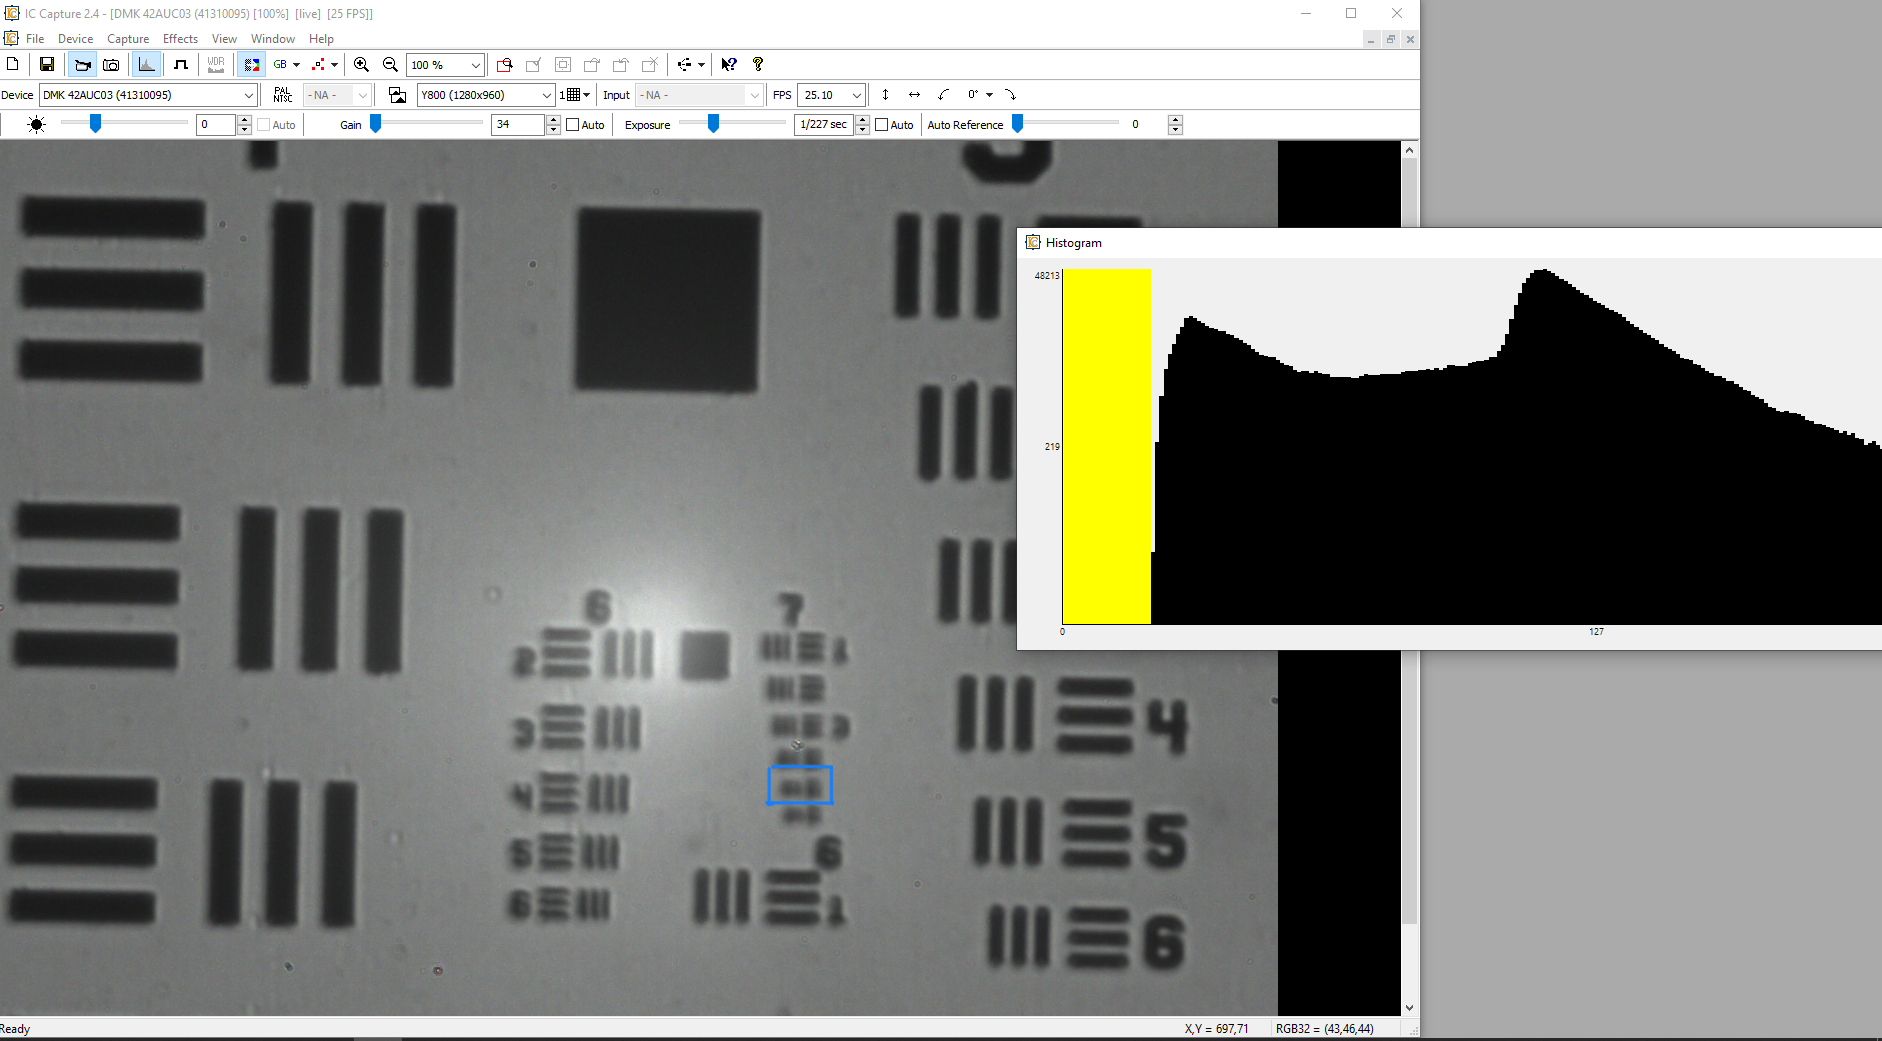
\includegraphics[width=\textwidth]{NAblau6mm}
		\captionbelowof{figure}{Testobjekt bei blauer LED \newline mit Blendendurchmesser von 6 mm}
		\label{fig:b_6}
	\end{minipage}
	\vspace{2mm}
	\begin{minipage}[t]{0.50\textwidth}
		\centering
		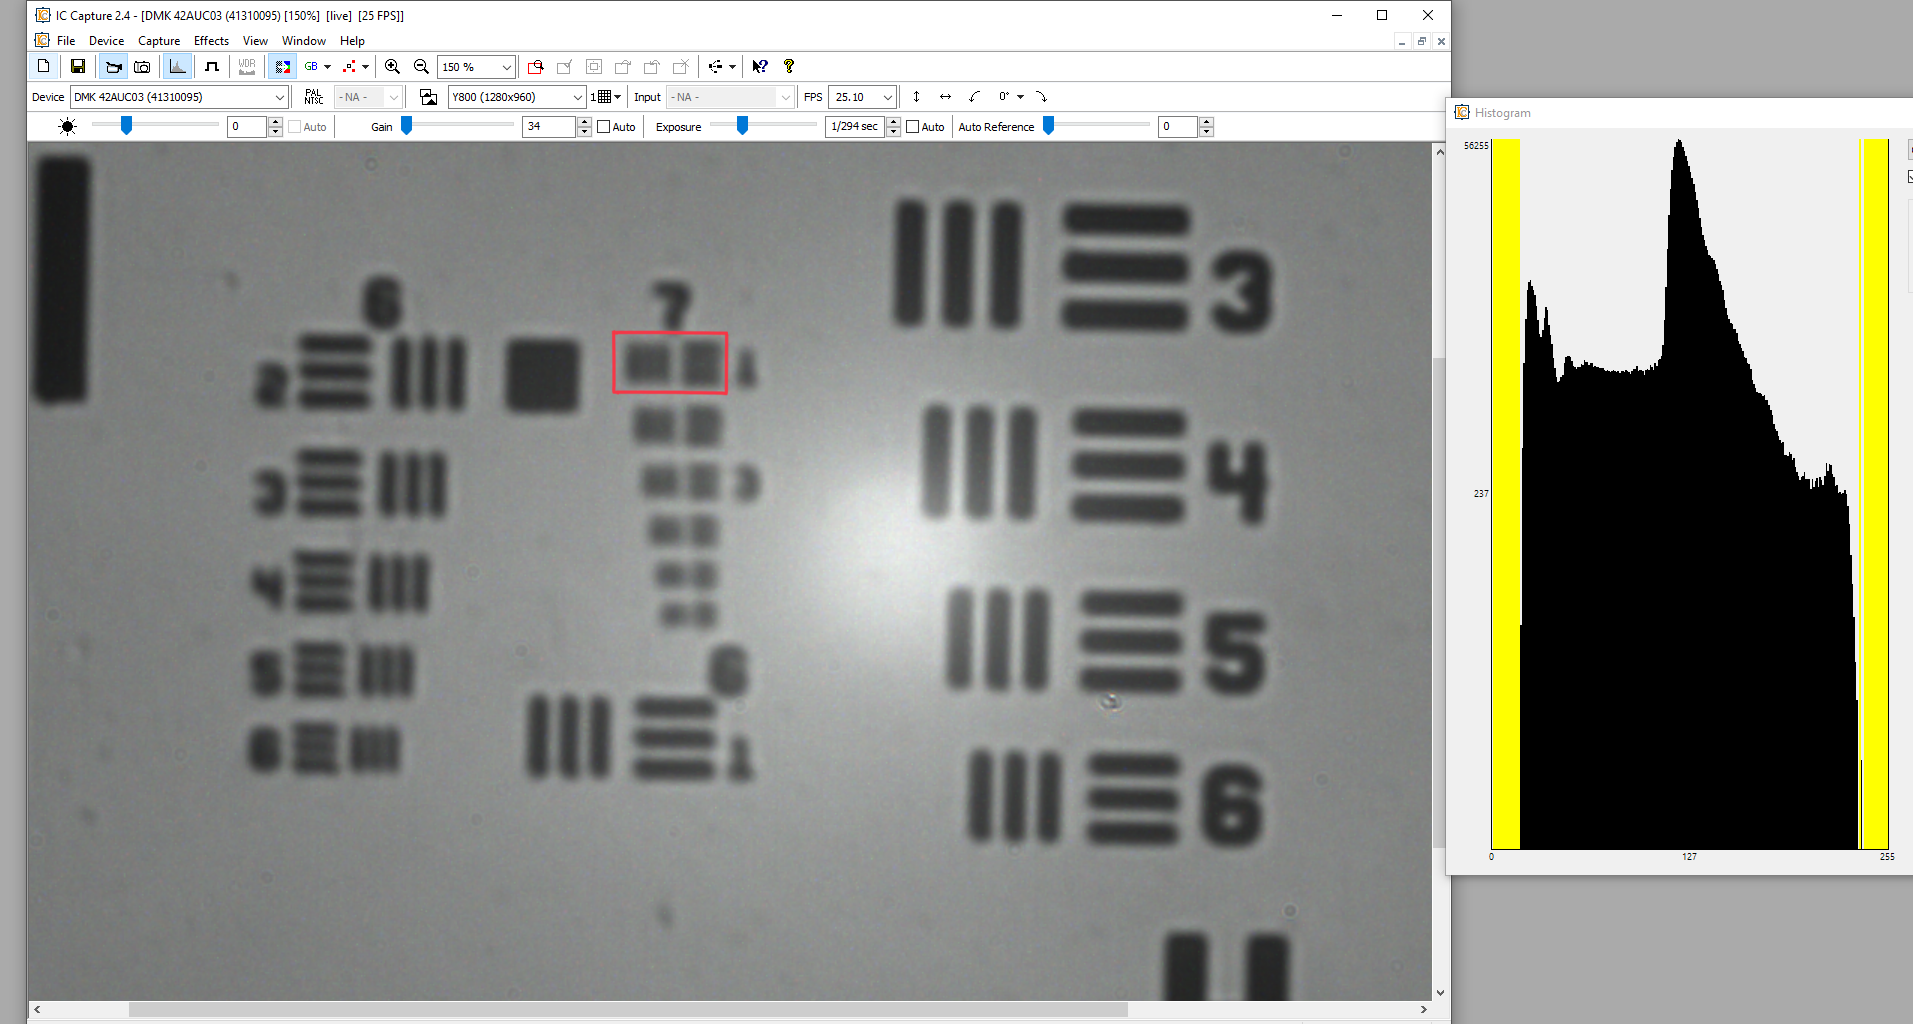
\includegraphics[width=\textwidth]{NAROT6mm}
		\captionof{figure}{Testobjekt bei roter LED \newline mit Blendendurchmesser von 6 mm}
		\label{fig:r_6}
	\end{minipage}
	\vspace{1em}
\end{minipage}

\noindent Nun wird der Blendendurchmesser auf 3 mm reduziert.

\vspace{2mm}

\begin{minipage}{\textwidth}
	\begin{minipage}[t]{0.5\textwidth}
		\centering
		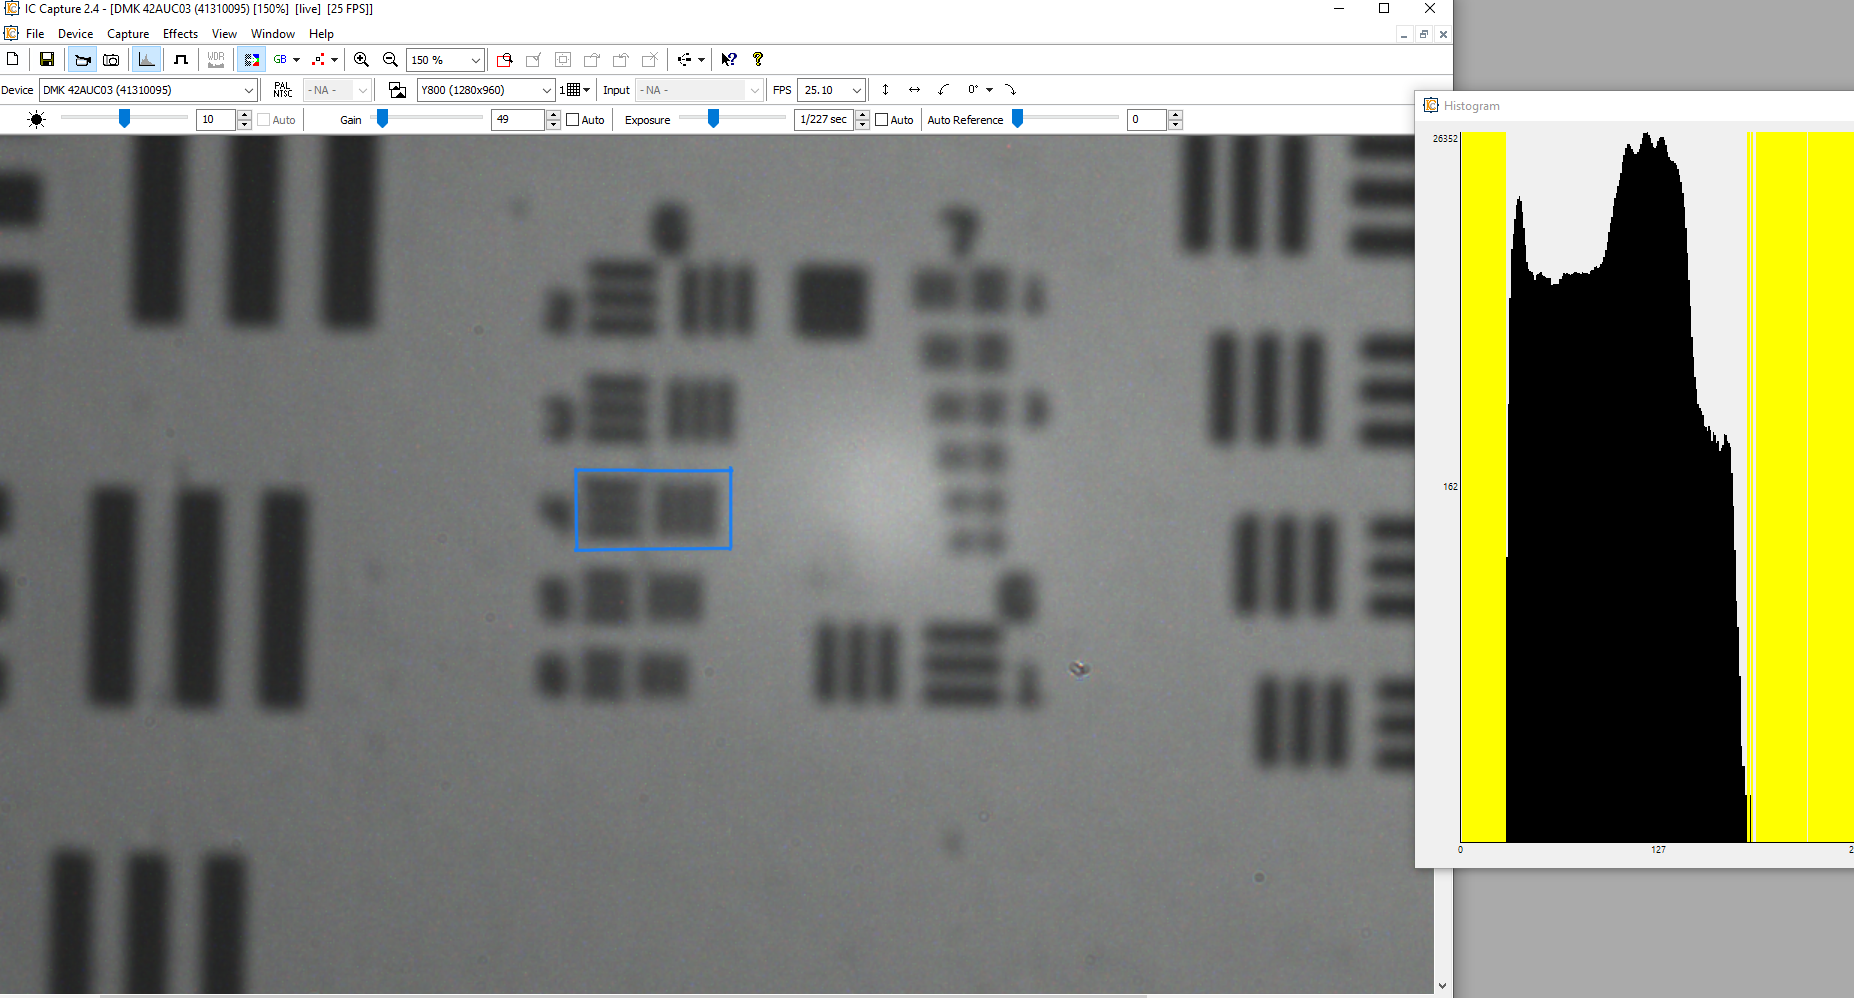
\includegraphics[width=\textwidth]{NAblau3mm}
		\captionbelowof{figure}{Testobjekt bei blauer LED \newline mit Blendendurchmesser von 3 mm}
		\label{fig:b_3}
	\end{minipage}
	\vspace{2mm}
	\begin{minipage}[t]{0.50\textwidth}
		\centering
		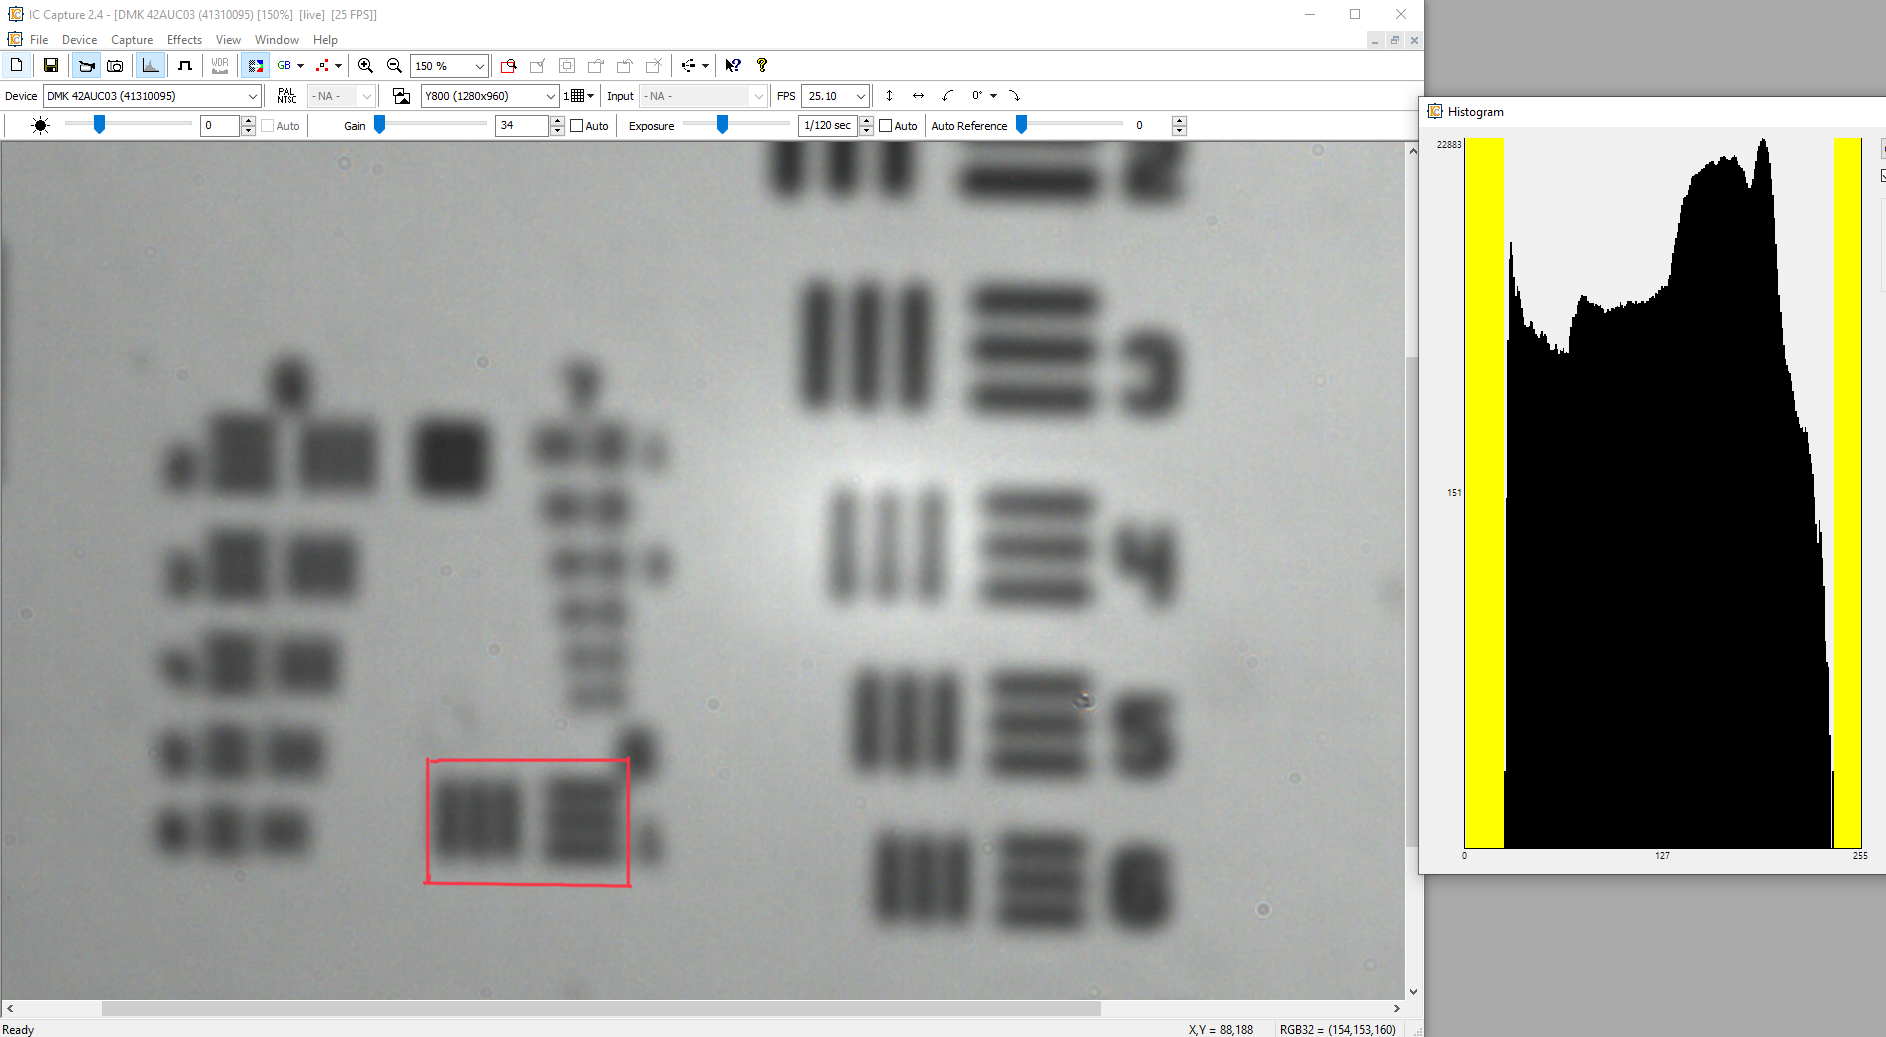
\includegraphics[width=\textwidth]{NAROT3mm}
		\captionof{figure}{Testobjekt bei roter LED \newline mit Blendendurchmesser von 3 mm}
		\label{fig:r_3}
	\end{minipage}
	\vspace{1em}
\end{minipage}

\newpage

\noindent Schließlich wird der gesamte Versuch auch noch mit einem Blendendurchmesser von 2 mm wiederholt.

\vspace{2mm}

\begin{minipage}{\textwidth}
	\begin{minipage}[t]{0.5\textwidth}
		\centering
		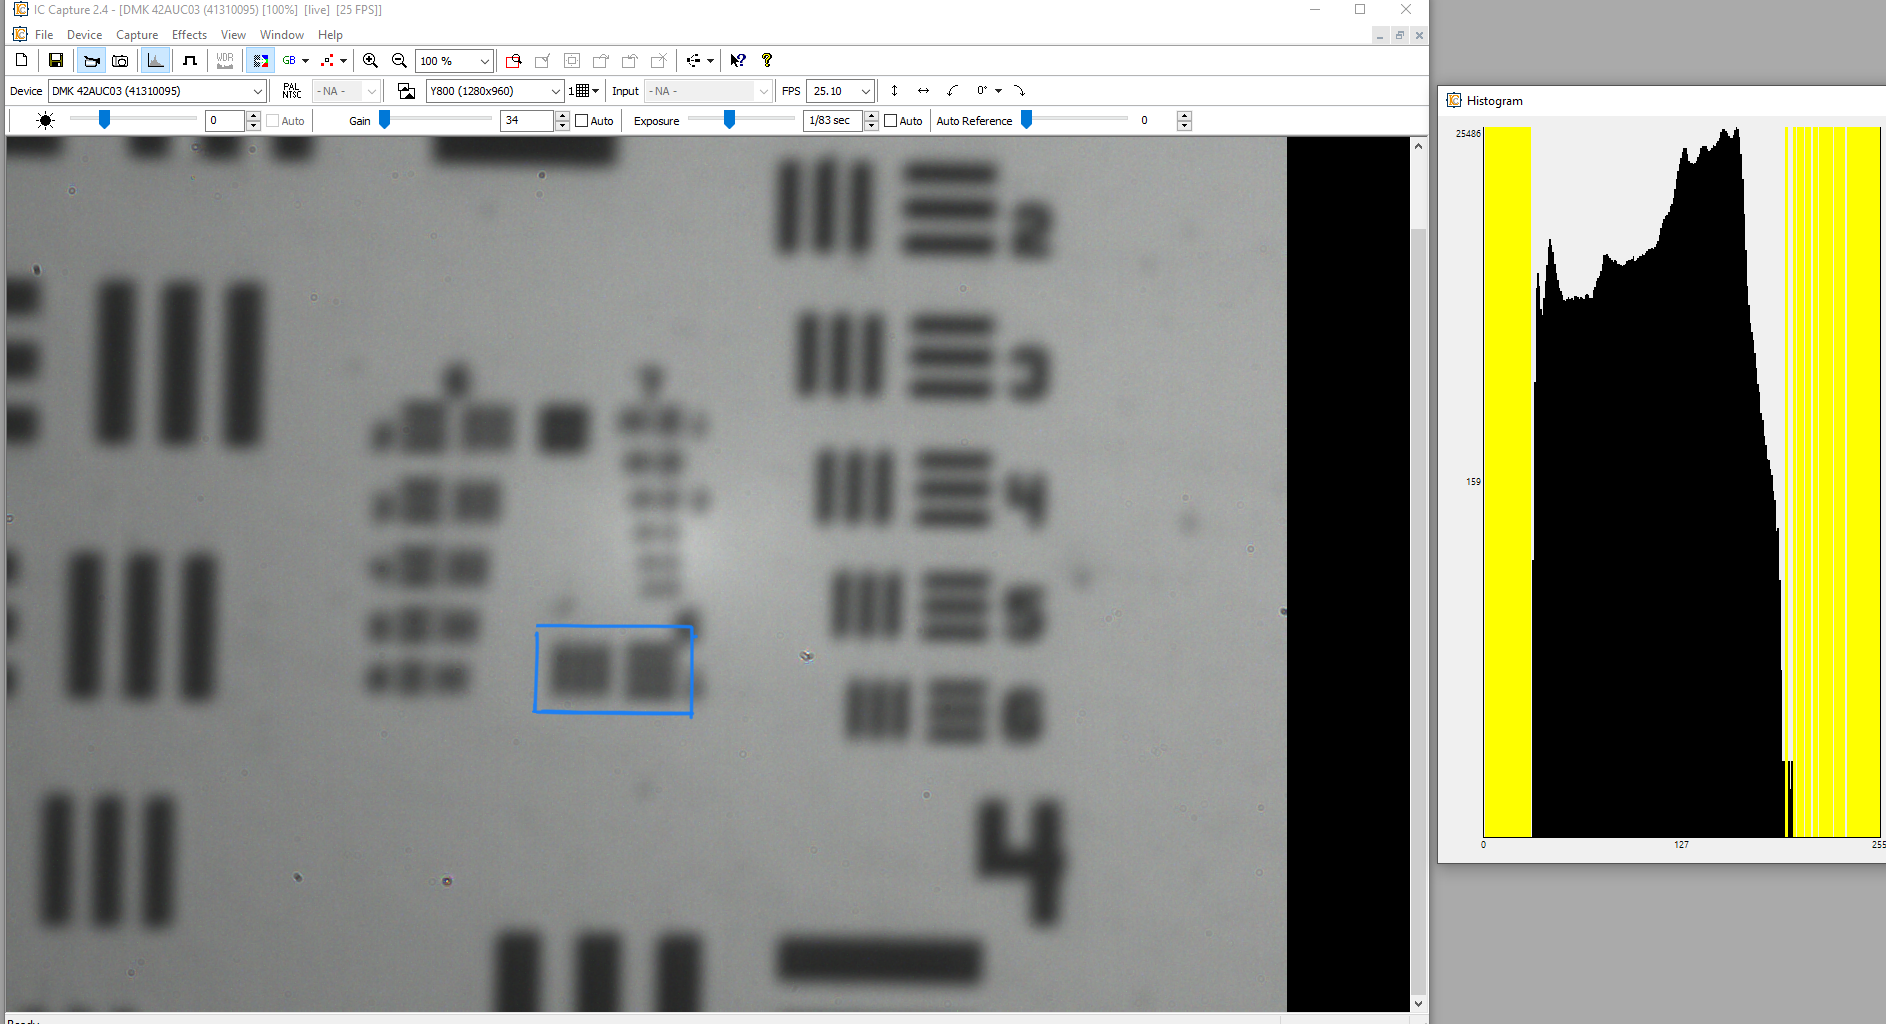
\includegraphics[width=\textwidth]{NAblau2mm}
		\captionbelowof{figure}{Testobjekt bei blauer LED \newline mit Blendendurchmesser von 2 mm}
		\label{fig:b_2}
	\end{minipage}
	\vspace{2mm}
	\begin{minipage}[t]{0.50\textwidth}
		\centering
		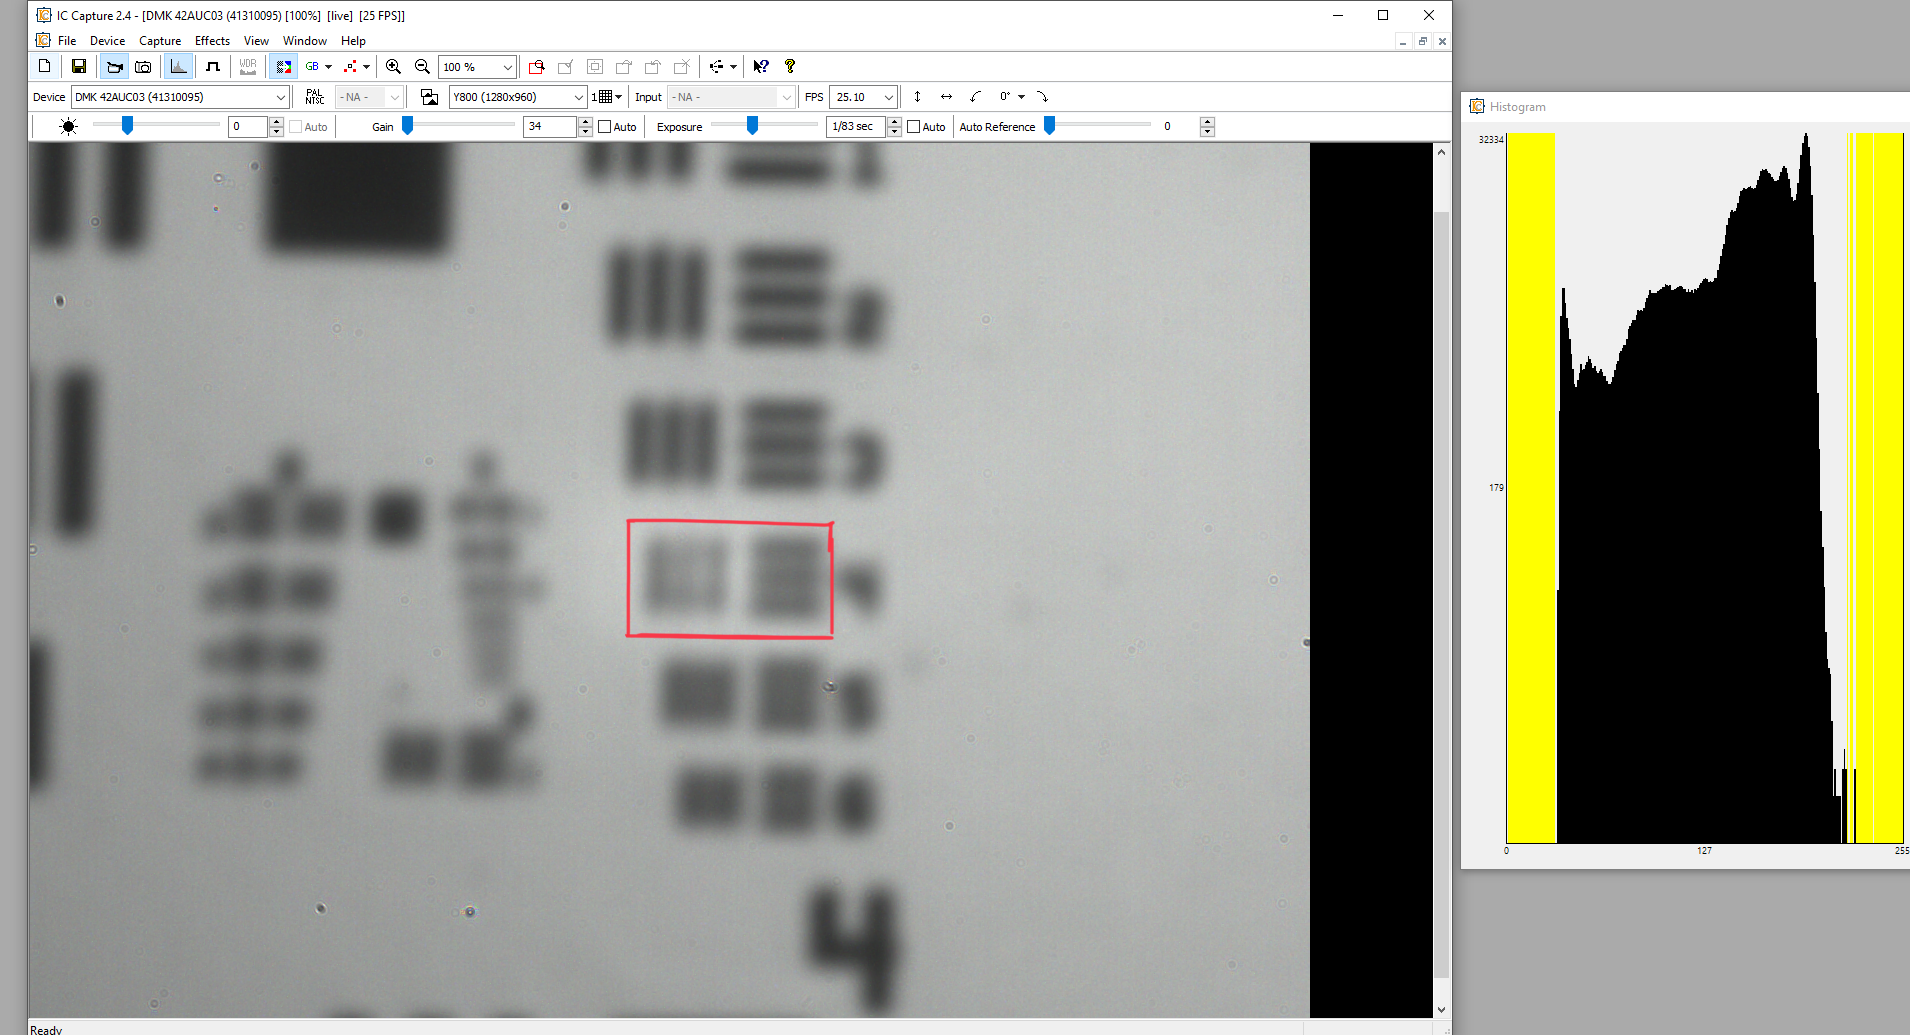
\includegraphics[width=\textwidth]{NAROT2mm}
		\captionof{figure}{Testobjekt bei roter LED \newline mit Blendendurchmesser von 2 mm}
		\label{fig:r_2}
	\end{minipage}
	\vspace{1em}
\end{minipage}

\noindent Zunächst werden für die gerade noch unterscheidbaren Balken die entsprechenden räumlichen Frequenzen anhand der Tabelle in \autoref{fig:tab} bestimmt. Zur besseren Übersicht wurden die entsprechenden Balken in den Abbildungen der Testobjekte schon markiert. Die erhaltenen Werte sind in folgender Tabelle aufgelistet. Als Unsicherheit wurde dabei die größere Differenz zum benachbarten Wert angenommen.

\renewcommand{\arraystretch}{1.2}
\begin{table}[H]
	\caption{ erhaltene Werte für die räumliche Frequenz\\ ||| \dots Striche  \\ $\xi$ \dots räumliche Frequenz  \\ $r$ \dots Blendenradius\\  $\lambda$ \dots Wellenlänge}
	\label{tab:werte}
	\begin{center}
		\begin{tabular}{S|S|S}
			{$\xi$ / \si{\strich\per\mm}} & {$r$ / \si{\mm}} & {$\lambda$ / \si{\nm}} \\ \hline
			200+-30                       & 3   +-  0.05     & 470+-5                 \\
			91+-12                        & 1.5 +-  0.05     & 470+-5                 \\
			60+-8                         & 1   +-  0.05     & 470+-5                 \\
			128+-16                       & 3.0 +-  0.05     & 635+-5                 \\
			64+-8                         & 1.5 +-  0.05     & 635+-5                 \\
			45+-6                         & 1   +-  0.05     & 635+-5                 \\
			\hline
		\end{tabular}
	\end{center}
\end{table}

\vspace{2mm}

\subsection{Zusatz - Dunkelfeldmikroskopie}

Dunkelfeldmikroskopie ist eine Variante der Lichtmikroskopie, bei der ein
dunkler Hintergrund mit hellen Konturen entsteht. Diese Art der Mikroskopie,
ist besonders bei lebenden, sich bewegenden, Präparaten vorteilhaft, weil so
auch bei geringen Kontrast und ohne Einfärbungen Strukturen sichtbar werden.

\newpage

Um das Phänomen der Dunkelfeldmikroskopie zu erreichen, muss dafür gesorgt
werden, dass kein direktes Licht in das Objektiv gelangt und nur das abgelenkte
Licht verwendet wird. \cite{wiki_dunkel_2021}

\vspace{2mm}

Um nun Dunkelfeldmikroskopie betreiben zu können, muss das direkte Licht
ausgeblendet werden. Dies wird mithilfe eines Drahts erreicht, der so in den
Lichtweg gedreht wird, dass die nullte Beugungsordnung verschwindet, wie in
\autoref{fig:dunkelf_beu} sichtbar.


Durch entfernen der Linse L3 wird wiederum das Bild sichtbar, das in \autoref{fig:dunkelf_bild} abgebildet ist.

\begin{minipage}{\textwidth}
	\begin{minipage}[t]{0.5\textwidth}
		\centering
		\includegraphics[width=\textwidth]{abbe/dunkelfeld_mustere}
		\captionbelowof{figure}{Beugungsbild mit ausgeblendeter nullter Ordnung}
		\label{fig:dunkelf_beu}
	\end{minipage}
	\vspace{2mm}
	\begin{minipage}[t]{0.50\textwidth}
		\centering
		\includegraphics[width=\textwidth]{abbe/dunkelfeld_bild}
		\captionof{figure}{Bild des Objekts bei ausgeblendeter nullter Ordnung}
		\label{fig:dunkelf_bild}
	\end{minipage}
	\vspace{1em}
\end{minipage}

Wie es die Theorie voraussagt, werden nur die Konturen sichtbar, während sich der Rest des Objekts nicht vom Hintergrund unterscheiden lässt.


\vspace{5mm}

\section{Auswertung}

\subsection{Zusammenhang zwischen der Auflösung und der Anzahl der Bergungsordnungen}

\noindent Wie anhand der Abbe-Theorie vorausgesagt, erkennt man bei direkten Vergleich der \autoref{fig:bild5} bis \autoref{fig:bild1}, dass die Auflösung des Bildes immer schlechter wird. Die Betrachtung von \autoref{fig:bild0} zeigt auch, dass nur anhand der Beugungsbilder 0-ter Ordnung, keine räumliche Auflösung möglich ist.

\newpage

\subsection{Auflösungsvermögen in Abhängigkeit von der N.A.}

Unter der Verwendung der Werte aus \autoref{tab:werte} und der \autoref{eq:na_approx} erhält man folgende Werte für die N.A.

%Tabelle NA
\begin{table}[H]
	\caption{ Erhaltene Werte für die nummerische Apertur\\ $N.A.$ \dots erhaltener Wert für die nummerische Apertur  \\ $\Delta N.A$ \dots erhaltene Unsicherheit der nummerische Apertur}
	\label{tab:na}
	\begin{center}

		\begin{tabular}{lrr}
			\toprule
			N.A.   & $\Delta $N.A. \\
			\midrule
			0.0500 & 0.0008        \\
			0.0250 & 0.0008        \\
			0.0167 & 0.0008        \\
			\bottomrule
		\end{tabular}
	\end{center}
\end{table}

Aus den Werten der \autoref{tab:werte} und der \autoref{eq:aufl_durch_xi} erhält man schließlich folgende Werte für das Auflösungsvermögen $d$.

%Tabelle Auflösungsvermögen
\begin{table}[H]
	\caption{ Erhaltene Werte für das Auflösungsvermögen\\ $d$ \dots Auflösungsvermögen in mm\\ $\Delta d$ \dots Unsicherheit des Auflösungsvermögens in mm}
	\label{tab:aufl}
	\begin{center}

		\begin{tabular}{lrr}
			\toprule
			$d $ / mm & $\Delta d $ / mm \\
			\midrule
			0.0078    & 0.0010           \\
			0.0156    & 0.0019           \\
			0.022     & 0.003            \\
			\bottomrule
		\end{tabular}
	\end{center}
\end{table}


Die Daten aus den so erzeugten \autoref{tab:na} und \autoref{tab:aufl} werden nun geplottet und eine theoretsche Fitkurve auf den Graphen angewendet, was folgende \autoref{fig:aufl_vergleich} erzeugt.

% Graph
\begin{figure}
	\begin{center}
		\includegraphics[width=0.95\textwidth]{./pics/aufl.png}
	\end{center}
	\caption{Gemessene Werte für das Auflösungsvermögen im Vergleich zu den theoretischen Kurven für blaues und rotes Licht}
	\label{fig:aufl_vergleich}
\end{figure}


\newpage

\section{Diskussion}\label{disk}

\subsection{Zusammenhang zwischen der Auflösung und der Anzahl der Bergungsordnungen}

Wie bereit erwähnt decken sich die erhaltenen Ergebnisse, mit jenen, die aufgrund der Abbe-Theorie vorausgesagt wurden. Allerdings lässt sich dieses Ergebnis nicht Quantifizieren, da keine einheitliche Metrik für die Verschwommenheit vorhanden ist.

\vspace{2mm}

\subsection{Auflösungsvermögen in Abhängigkeit von der N.A.}

Wie in \autoref{fig:aufl_vergleich} ersichtlich, ist der theoretische Verlauf von der N.A. zum Auflösungsvermögen im Fehlerintervall der gemessenen Werte enthalten. Es ist allerdings zu beachten, dass die Unsicherheiten, mit $\pm$ einem Element aus der Tabelle, großzügig gewählt worden sind, da die Wahrnehmung der getrennten Balken sehr subjektiv ist und daher bei unterschiedlichen Experimentatoren leicht zu anderen Ergebnissen führen kann.

\vspace{5mm}

\section{Zusammenfassung}

Die erhaltenen Ergebnisse decken sich mit der vorhergesagten Theorie. Allerdings ist dabei anzumerken, dass die meisten Messungen auf subjektiven Wahrnehmungen beruhen und daher keine absoluten Aussagen getroffen werden können.

\newpage

\section{Anhang}

Hier im Anhang befindet sich nochmals der Strahlengang, der als Vorbereitung zu zeichnen war.

\vspace{2mm}

\begin{figure}[H]
	\begin{center}
		\includegraphics[width=0.5\textwidth]{anhang_abbe}
	\end{center}
	\caption{gezeichneter Strahlengang}
	\label{fig:zeich}
\end{figure}

\newpage

\printbibliography
\listoffigures
\listoftables
\end{document}



%Vorlagen
%

%Gleichungen werden so oder mit \begin{equation} formatiert

%Zitate
%\cite{erstes Wort}


%Unterdrücken von Einrücken
%\noindent 

%referenzen
% \aotoref{name}

%für Formeln $ f $
%\subsection{Idealisierungen}

%Gleichung

%\begin{equation}
%	k_{pos} = \frac{4}{300} \frac{V}{\mu\mathrm{s}} = 13333 \, \frac{V}{s}
%\end{equation}

%\begin{align}
%	 \ddot \phi -\frac{g}{l} \cdot \phi &=0 \label{eq:harm}\\
%     \frac{\text{d}^{2}}{\text{dt}^{2}} [\sin(\omega t)]  - \frac{g}{l} \cdot \sin(\omega t) &= 0 \\ 
%     \therefore \quad \omega^{2}&=\frac{g}{l} \label{eq:omega}
%\end{align}


%\begin{align}
%    T &= 2\pi \sqrt{\frac{l}{g}} \label{eq:reg_sqrt} \\
%    T^{2} &= \frac{4\pi^{2}}{g} l \label{eq:reg_lin} 
%\end{align}

%Kompliziertes Bild

%\begin{minipage}{\textwidth}
%\begin{minipage}[t]{0.43\textwidth}
%	\includegraphics[width=\textwidth]{pics/toplot.PNG}
%\end{minipage}
%\begin{minipage}[t]{0.45\textwidth}
%	\includegraphics[width=\textwidth]{pics/bottomlot.PNG}
%\end{minipage}
%	\captionof{figure}{Ansicht von Oben (Rechts) und von Unten (Links) des Senklots}
%	\label{fig:Senklot}
%    \vspace{1em}
%\end{minipage}



%\begin{minipage}{\textwidth}
%\begin{minipage}[t]{0.59\textwidth}
%    \centering
%    \includegraphics[width=\textwidth]{pics/Aufhangung.jpeg}
%    \captionbelowof{figure}{Aufhängung}
%    \label{fig:Aufhaengung}
%\end{minipage}
%\begin{minipage}[t]{0.40\textwidth}
%    \centering
%    \includegraphics[width=\textwidth]{pics/PendelAufbau.png}
%    \captionof{figure}{Versuchsaufbau}
%    \label{fig:Aufbau}
%\end{minipage}
%    \vspace{1em}
%\end{minipage}

%\begin{wrapfigure}[]{r}{0.4\textwidth}
%\begin{tabular}{@{}l@{}}
%\begin{minipage}{\textwidth}
%\includegraphics[width=0.38\textwidth]{pics/Aufhangung.jpeg}
%\noindent \captionbelowof{figure}{Aufhängung}
%\label{fig:Aufhaengung}
%\end{minipage}\\
%\begin{minipage}{\textwidth}
%\includegraphics[width=0.38\textwidth]{pics/PendelAufbau.png}
%\captionof{figure}{Versuchsaufbau}
%\label{fig:Aufbau}
%\end{minipage}
%\end{tabular}
%\end{wrapfigure}


%Tabelle

%\begin{align}
%	\Delta \bar T_{10} &= t \sigma_{\bar T_{10}} + \Delta T_{res} = \frac{t}{\sqrt{N}}\sigma_{T_{10}}+\Delta T_{res}\\
%	\Delta \bar T &= \frac{ \Delta \bar T_{10}}{10}
%\end{align}


%Tabelle
%
%\begin{table}[htbp]
%\centering
%\begin{tabular}{c|c|c|c|l}
%    [$\frac{\text{m}}{\text{s}^{2}}$] & Literaturwert & Wurzel Fit & Linearer Fit &\\ \hline
%    $g$ & \num{9.806191} & \num{9.79} & \num{9.80} &\\
%    $\Delta g$ & \num{1.2e-5} & \num{1e-2}& \num{1e-2} &\\
%\end{tabular}
%	\captionbelowof{table}{Vergleich mit Literaturwert}
%	\label{Tab:Vergleich}
%\end{table}


%\begin{align}
%	& \Delta T_{\phi} = 2\pi \sqrt{ \frac{l}{g} } \frac{\phi^{2}}{16} = 0.0052\,\text{s} 
%\end{align}
